% translate_docs: ./cars/E-GMP_gen1/Ioniq5/head_unit_preconditioning_kit_Ioniq5_install.tex @ 1310963db16097b8980375704a3fc258a6de4b75
\documentclass[superscriptaddress,onecolumn,floatfix]{revtex4-2}

\usepackage{graphicx}
\usepackage{epsfig}
\usepackage{color}
\usepackage{amssymb}
\usepackage{amsmath}
\usepackage{array}
\usepackage[loose]{units}
\usepackage[colorlinks=true]{hyperref}
\usepackage{cleveref}
\usepackage{braket}
\usepackage[caption=false]{subfig}
\usepackage[german]{babel}
\usepackage{letltxmacro}

\pdfcompresslevel=9

\LetLtxMacro{\ORIGselectlanguage}{\selectlanguage}
\makeatletter
\DeclareRobustCommand{\selectlanguage}[1]{%
    \@ifundefined{alias@\string#1}
      {\ORIGselectlanguage{#1}}
      {\begingroup\edef\x{\endgroup
         \noexpand\ORIGselectlanguage{\@nameuse{alias@#1}}}\x}%
}
\newcommand{\definelanguagealias}[2]{%
  \@namedef{alias@#1}{#2}%
}
\makeatother

\definelanguagealias{de}{german}


\begin{document}
\selectlanguage{de}

\begin{abstract}
  Diese Anleitung führt Sie durch die notwendigen Schritte zur Installation des Vorkonditionierungskits für das Autoradio in Ihrem Ioniq 5 (Modelljahre 2021–2024). Siehe auch \href{https://youtube.com/playlist?list=PLYCTmVJH4UYqnw87UZAaqMo1GrOv0cJaL}{Videoanleitungen}:
  \begin{description}
    \item[Schritt 1: 12V-Anschluss trennen] Videoanleitung: \href{https://youtu.be/ePBdyeBYKk4}{https://youtu.be/ePBdyeBYKk4}
    \item[Schritt 2: Trimmen: Option A] Lange und sorgfältige Videoanleitung zum Trimmen: \href{https://youtu.be/nE4CqGsin7Q}{https://youtu.be/nE4CqGsin7Q}
    \item[Schritt 2: Trimmen: Option B] Schnelle und einfache Videoanleitung zum Trimmen: \href{https://youtu.be/291boryx-Vc}{https://youtu.be/291boryx-Vc}
    \item[Schritt 3: Kabelbaumanschluss] Videoanleitung: \href{https://youtu.be/JgrhReAnDGc}{https://youtu.be/JgrhReAnDGc}
    \item[Schritt 4: OBD-Halterung] Videoanleitung: \href{https://youtu.be/PqwYul43jFw}{https://youtu.be/PqwYul43jFw}
  \end{description}
\end{abstract}
\title{Installationsanleitung für das Vorkonditionierungsset}
\author{Electroniq Buttons Boutique}
\email{support@electroniqbuttons.com}
% \affiliation{\GOE}
% \author{Benjamin J. McMorran}
% \email{mcmorran@uoregon.edu}
% \affiliation{\UO}
\date{\today}

\maketitle

\begin{figure}[h]
  \subfloat[]{\label{subfig:overview:harness}
  \includegraphics[height=1.95in]{../../../harnesses/head_unit_MITM/photos/whole_harness.jpg} } \\
  \subfloat[]{\label{subfig:overview:trim}
  \includegraphics[width=6in]{photos/overview_labeled.jpg} }
   \caption{(a) Mann-in-der-Mitte-Gurt. (b) Übersicht der beteiligten Verkleidungsteile. \label{fig:overview}}
\end{figure}

\section{Einführung}
  Diese Anleitung dient dazu, die schrittweise Installation des Vorkonditionierungskits für das Steuergerät bzw. des in Abbildung 1 dargestellten Kabelbaums für die Steuereinheit (Man-in-the-Middle-Kabelbaum) zu veranschaulichen. \ref{subfig:overview:harness}Im Abschnitt \ref{sect:1}Wir stellen zwei Möglichkeiten zum Entfernen der Verkleidung vor, um Zugang zum Hauptgerät zu erhalten. In Abschnitt \ref{sect:2}In Abschnitt 1 beschreiben wir den Vorgang des Anschließens des Kabelbaums. \ref{sect:3}Wir zeigen den Anschluss des OBD-Anschlusses und wie man den Mikrocontroller einsteckt. 

Erforderliche Werkzeuge:
\begin{enumerate}
  \item 10-mm-Steckschlüssel oder verstellbarer Schraubenschlüssel für 12-V-Batterie (nicht im Lieferumfang enthalten).
  \item Werkzeuge zum Entfernen der Zierleisten (bei Auswahl enthalten)
  \item Phillips \#2 Inbusschlüssel (im Lieferumfang enthalten, falls ausgewählt) oder ähnliches
\end{enumerate}

Kit-Bestandteile:
\begin{enumerate}
  \item Kabelbaum für das Hauptgerät
  \item WiCAN
  \item 70-mm-OBD-Halterung
  \item 70 mm doppelseitiges Klebeband (zwei Stücke zur Sicherheit enthalten)
  \item 4 Kabelbinder
\end{enumerate}

\section{Schritt 1: Den Minuspol der 12-V-Batterie abklemmen.} \label{sect:0}
Trennen Sie immer zuerst die 12-V-Batterie, bevor Sie irgendwelche elektrischen Steckverbinder entfernen! Das Entfernen eines stromführenden Steckers kann eine Entladung verursachen und einen Stecker oder das Steuergerät Ihres Autos zerstören.

Schritt-für-Schritt-Anleitung:
\begin{enumerate}
  \item Motorhaube öffnen (Abbildung \ref{subfig:12V:hood})
  \item Öffnen Sie den Frunk. 
  \item Entfernen Sie die Abdeckung für die 12-V-V-Schnittstelle (Abbildung \ref{subfig:12V:panel})
  \item Die Mutter auf der negativen Seite mit einer 10-mm-Nuss lösen (Abbildung \ref{subfig:12V:nut})
  \item Entfernen Sie den Minuspol (Abbildung \ref{subfig:12V:terminal})
\end{enumerate}

\begin{figure}[h]
  \subfloat[]{\label{subfig:12V:hood}
  \includegraphics[height=1.5in]{photos/open_hood.jpg} } 
  \subfloat[]{\label{subfig:12V:panel}
  \includegraphics[height=1.5in]{photos/remove_panel.jpg} }  \\
  \subfloat[]{\label{subfig:12V:nut}
  \includegraphics[height=1.5in]{photos/loosen_nut.jpg} } 
  \subfloat[]{\label{subfig:12V:terminal}
  \includegraphics[height=1.5in]{photos/disconnect_terminal.jpg} } 
   \caption{(a) Öffnen Sie die Motorhaube. (b) Entfernen Sie die Abdeckung des 12-V-Anschlusses. (c) Lösen Sie die Mutter am Minuspol. (d) Entfernen Sie den Minuspol. \label{fig:12V}}
\end{figure}

\section{Schritt 2: Zuschneiden} \label{sect:1}
Ziel ist es, an das Herzstück des Geräts zu gelangen: das Hauptsteuergerät. Der korrekte Weg erfordert das Entfernen von vier Verkleidungsteilen und der AVN-Tastatur (Klimabedienleiste). Es gibt auch eine Abkürzung. Diese ist zwar deutlich schneller, aber umständlicher und birgt ein höheres Risiko, sich an einer scharfen Kante der Verkleidung zu verletzen. Wählen Sie die Methode, die Ihnen am besten passt.
\begin{figure}[h]
  \subfloat[]{\label{subfig:step1:X}
  \includegraphics[height=2.95in]{photos/overview_X.jpg} } 
   \caption{Das X markiert das Hauptgerät. \label{fig:step1}}
\end{figure}

\begin{figure}[h]
  \subfloat[]{\label{subfig:trim:lower}
  \includegraphics[height=1.5in]{photos/crash_pad_lower.jpg} } 
  \subfloat[]{\label{subfig:trim:airvent}
  \includegraphics[height=1.5in]{photos/crash_pad_air_vent.jpg} } 
  \subfloat[]{\label{subfig:trim:center}
  \includegraphics[height=1.5in]{photos/crash_pad_center_and_keyboard.jpg} } 
   \caption{(a) Untere Seite des Crashpads. (b) Lüftungsschlitz des Crashpads. (c) Zierleiste des Crashpads, AVN-Tastatur und Mitte des Crashpads. \label{fig:trim}}
\end{figure}

\subsection{Option A: lang und sorgfältig}
Reihenfolge der Arbeitsschritte beim Verkleiden: 
\begin{enumerate}
  \item Sturzpad unten (Abbildung \ref{subfig:trim:lower}) \label{step:cpl}
  \item Belüftungsöffnung des Crashpads (Abbildung \ref{subfig:trim:airvent}) \label{step:cpav}
  \item Crashpad-Garnitur (Abbildung \ref{subfig:trim:center})
  \item AVN-Tastatur (Abbildung \ref{subfig:trim:center})
  \item Mitte des Crashpads (Abbildung \ref{subfig:trim:center})
\end{enumerate}

Schritte \ref{step:cpl} Und \ref{step:cpav} Die Reihenfolge der Schritte ist beliebig; beide Schritte müssen jedoch durchgeführt werden, um die Verkleidung der Crashpads zu lösen.

Schritt-für-Schritt-Anleitung:
\begin{enumerate}
  \item Schraube im unteren Teil des Sturzpads entfernen (Abbildung \ref{subfig:trimsteps:lowerscrew})
  \item Die rechte Hälfte der unteren Crashpad-Abdeckung lässt sich mithilfe von Verkleidungsdemontagewerkzeugen entfernen.
  \item Entfernen Sie währenddessen die Schraube(n) hinter der unteren Sturzpolsterung (möglicherweise 1 oder 2; siehe Abbildung). \ref{subfig:trimsteps:cpc_llscrews}Die ganz links stehende Schraube am Lüftungsgitter dahinter neigt dazu, festzusitzen, daher muss man daran ziehen, um sicherzustellen, dass sie herausgedreht ist (Abbildung 1). \ref{subfig:trimsteps:cpc_llscrew})
  \item Entfernen Sie die Lüftungsöffnung des Crashpads.
  \item Entfernen Sie die Schraube, die sich hinter der Lüftungsöffnung des Crashpads befand (Abbildung 1). \ref{subfig:trimsteps:cpg_r_screw})
  \item Entfernen Sie die Verkleidung des Crashpads.
  \item AVN-Tastatur abnehmen 
    \begin{enumerate}
      \item Linke Schraube entfernen (Abbildung \ref{subfig:trimsteps:keyboard_l_screw})
      \item Rechte Schraube entfernen (Abbildung \ref{subfig:trimsteps:keyboard_ur_screw})
      \item Die untere linke Schraube entfernen (Abbildung \ref{subfig:trimsteps:keyboard_ll_screw})
      \item Die untere rechte Schraube entfernen (Abbildung \ref{subfig:trimsteps:keyboard_lr_screw})
      \item (Optional, prüfen Sie, ob keine 12-V-Stromversorgung vorhanden ist.) Entfernen Sie alle elektrischen Anschlüsse von der Rückseite der AVN-Tastatur.
      \item Die Zierclips durch Herausziehen der Tastatur lösen (Abbildung \ref{subfig:trimsteps:remove_keyboard})
      \item Falls die elektrischen Steckverbinder noch angeschlossen sind, vermeiden Sie es, zu viel Zug darauf auszuüben.
    \end{enumerate}
  \item Entfernen Sie die Schraube in der Mitte der oberen rechten Ecke des Crashpads, die durch die AVN-Tastatur blockiert war (Abbildung 1). \ref{subfig:trimsteps:cpc_urscrew})
  \item (optional) Stecken Sie die AVN-Tastatur zur sicheren Aufbewahrung wieder ein, falls die elektrischen Anschlüsse noch befestigt sind.
  \item Entfernen Sie die obere linke Schraube in der Mitte des Crashpads (Abbildung). \ref{subfig:trimsteps:cpc_ulscrew})
  \item Entfernen Sie die mittlere Verkleidung des Crashpads mithilfe von Verkleidungsdemontagewerkzeugen.
  \item (Prüfen Sie zuerst, ob keine 12-V-Spannung anliegt.) Trennen Sie den elektrischen Stecker an der Rückseite des Bedienfelds und entfernen Sie es aus dem Arbeitsbereich.
\end{enumerate}

\begin{figure}[h]
  \subfloat[]{\label{subfig:trimsteps:lowerscrew}
  \includegraphics[height=1.5in,angle=180]{photos/crash_pad_lower_screw.jpg} } 
  \subfloat[]{\label{subfig:trimsteps:cpc_llscrews}
  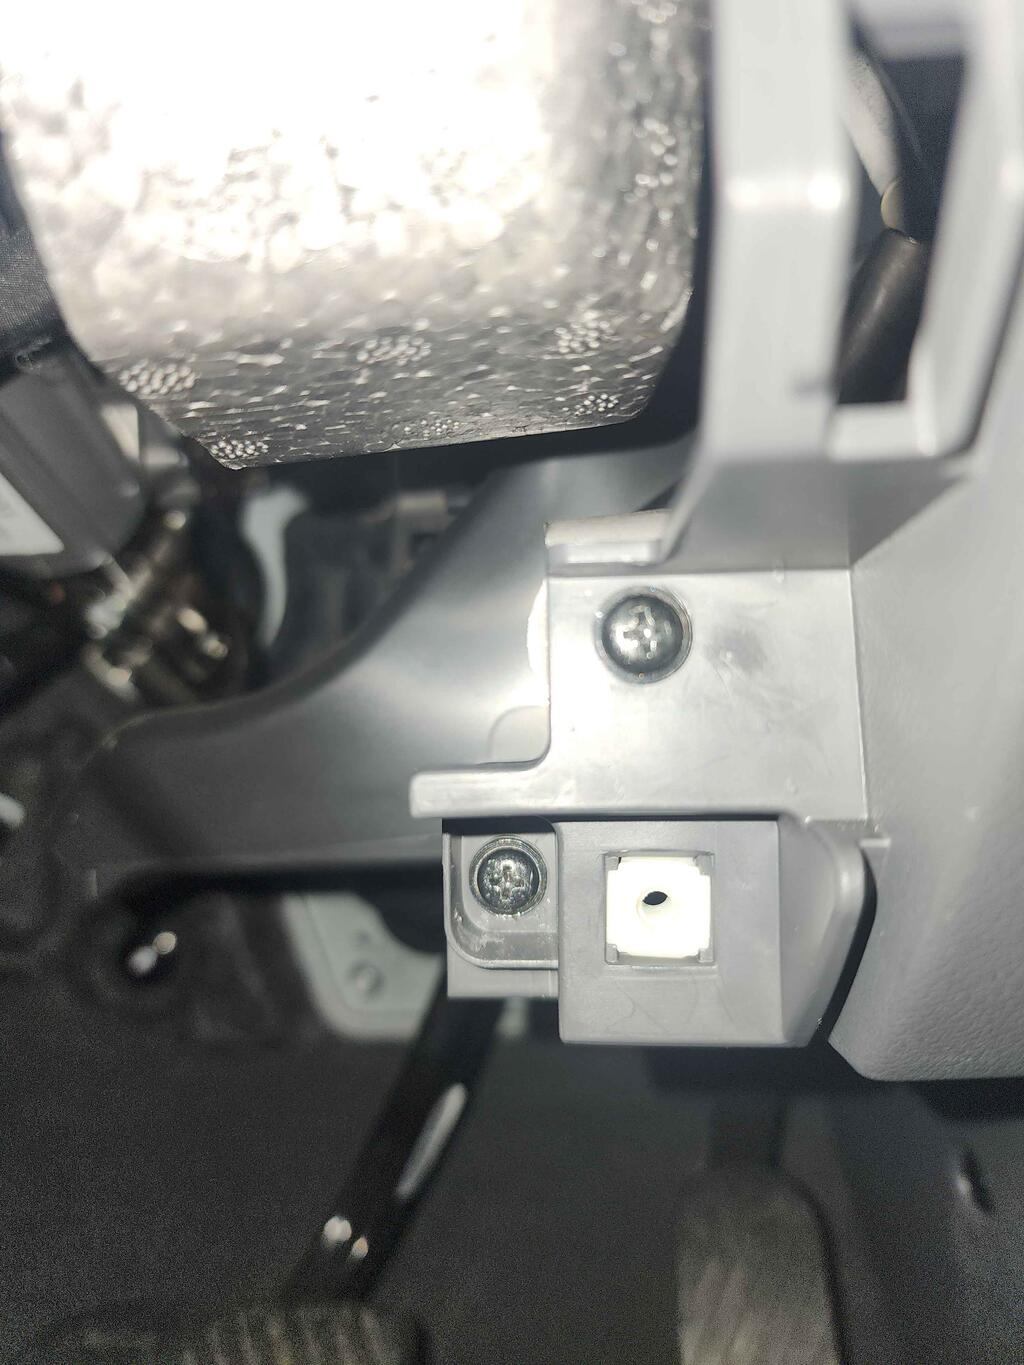
\includegraphics[height=1.5in,angle=180]{photos/crash_pad_center_ll_screws_3.jpg} } 
  \subfloat[]{\label{subfig:trimsteps:cpc_llscrew}
  \includegraphics[height=1.5in,angle=180]{photos/crash_pad_center_ll_screw.jpg} } 
  \subfloat[]{\label{subfig:trimsteps:cpg_r_screw}
  \includegraphics[width=1.5in,angle=-90]{photos/crash_pad_garnish_r_screw.jpg} }  \\
  \subfloat[]{\label{subfig:trimsteps:keyboard_l_screw}
  \includegraphics[height=1.5in,angle=180]{photos/keyboard_left_screw.jpg} } 
  \subfloat[]{\label{subfig:trimsteps:keyboard_ur_screw}
  \includegraphics[width=1.5in,angle=-90]{photos/keyboard_ur_screw.jpg} } 
  \subfloat[]{\label{subfig:trimsteps:keyboard_ll_screw}
  \includegraphics[height=1.5in,angle=180]{photos/keyboard_ll_screw.jpg} }  \\
  \subfloat[]{\label{subfig:trimsteps:keyboard_lr_screw}
  \includegraphics[height=1.5in,angle=0]{photos/keyboard_lr_screw.jpg} } 
  \subfloat[]{\label{subfig:trimsteps:remove_keyboard}
  \includegraphics[height=1.5in,angle=0]{photos/remove_keyboard.jpg} }  \\
  \subfloat[]{\label{subfig:trimsteps:cpc_urscrew}
  \includegraphics[width=1.5in,angle=-90]{photos/crash_pad_center_ur_screw.jpg} }  
  \subfloat[]{\label{subfig:trimsteps:cpc_ulscrew}
  \includegraphics[width=1.5in,angle=-90]{photos/crash_pad_center_ul_screw.jpg} } 
   \caption{(a) Schraube an der Unterseite des Crashpads entfernen. (b) Möglicherweise befinden sich ein oder zwei Schrauben hinter der Unterseite des Crashpads. (c) Schraube(n) hinter der Unterseite des Crashpads entfernen. (d) Schraube der Crashpad-Abdeckung entfernen. (e) Linke Schraube der AVN-Tastatur entfernen. (f) Rechte Schraube der AVN-Tastatur entfernen. (g) Linke Schraube unten an der AVN-Tastatur entfernen. (h) Rechte Schraube unten an der AVN-Tastatur entfernen. (i) AVN-Tastatur entfernen. (j) Mittlere Schraube des Crashpads entfernen, die von der AVN-Tastatur verdeckt wurde. (k) Mittlere Schraube des Crashpads entfernen, die sich hinter der Crashpad-Abdeckung links neben der AVN-Tastatur befand. \label{fig:trimsteps}}
\end{figure}
\subsection{Option B: schnell}
Bei dieser Vorgehensweise werden zwei Verkleidungsteile nur teilweise entfernt:
\begin{enumerate}
  \item Crashpad unten
  \item Crashpad-Mitte
\end{enumerate}
Beachten Sie, dass sich die Verkleidung des Crashpads während der Montage möglicherweise lösen kann. Sie kann nach der Montage einfach wieder angebracht werden.

Schritt-für-Schritt-Anleitung:
\begin{enumerate}
  \item Schraube im unteren Teil des Sturzpads entfernen (Abbildung \ref{subfig:trimsteps:lowerscrew})
  \item Die rechte Hälfte der unteren Crashpad-Abdeckung kann mit dem Verkleidungsdemontagewerkzeug entfernt werden. 
  \item Entfernen Sie währenddessen die Schraube(n) hinter der unteren Sturzpolsterung (möglicherweise 1 oder 2; siehe Abbildung). \ref{subfig:trimsteps:cpc_llscrews}Die ganz links stehende Schraube am Lüftungsgitter dahinter neigt dazu, festzusitzen, daher muss man daran ziehen, um sicherzustellen, dass sie herausgedreht ist (Abbildung 1). \ref{subfig:trimsteps:cpc_llscrew})
  \item Ziehen Sie den unteren Teil der Crashpad-Mitte heraus.
  \item Sie können nun von unterhalb der Crashpad-Mitte auf die Steuereinheit zugreifen.
\end{enumerate}

\subsection{Option C: Schnelle Option 2}

Diese Methode wird nicht empfohlen, sondern hier nur zur Information aufgeführt. Gründe, sie zu vermeiden:
\begin{enumerate}
  \item Benötigt einen langen geraden Schraubendreher für die 10-mm-Nuss.
  \item Bietet keinen so guten Zugang wie Option B (könnte aber mit Option B kombiniert werden).
  \item Die Wiedermontage der Zierleisten gestaltet sich schwieriger; die Ausrichtung der 3 Clips oben ist eine Herausforderung. 
\end{enumerate}
Der Hauptvorteil dieser Methode liegt darin, dass gut versteckte Montagepunkte möglich sind. Diese sind hier nicht dokumentiert, aber die \href{https://github.com/tylerharvey/Ioniq5_CAN/blob/main/guides/cars/E-GMP_gen1/EV6/head_unit_preconditioning_kit_EV6_install.pdf}{EV6 Installationsanleitung} bietet einige Ideen. Bei dieser Methode entfernen wir die untere mittlere Ablage des Crashpads sowie das Gehäuse für den vorderen USB-Anschluss. 

\begin{enumerate}
  \item Den linken Zierclip mit dem Zierleistenentfernungswerkzeug entfernen (Abbildung \ref{subfig:usb_trim:left_clip})
  \item Entfernen Sie den rechten Zierclip mit dem Zierleistenentfernungswerkzeug (Abbildung \ref{subfig:usb_trim:right_clip})
  \item Entfernen Sie den Boden des Konsolenfachs mit dem Verkleidungsdemontagewerkzeug (Abbildung \ref{subfig:usb_trim:carpet}) 
  \item Schraube mit einer 10-mm-Nuss auf einem langen Schlitzschraubendreher entfernen (Abbildung \ref{subfig:usb_trim:bolt})
  \item Hebeln Sie die Oberseite der unteren Ablage des Crashpads ab, um die 3 Zierclips an der Oberseite zu lösen (Abbildung \ref{subfig:usb_trim:trim_off})
  \item Legen Sie es beiseite (Abbildung \ref{subfig:usb_trim:trim_to_side})
\end{enumerate}

\begin{figure}[h]
  \subfloat[]{\label{subfig:usb_trim:left_clip}
  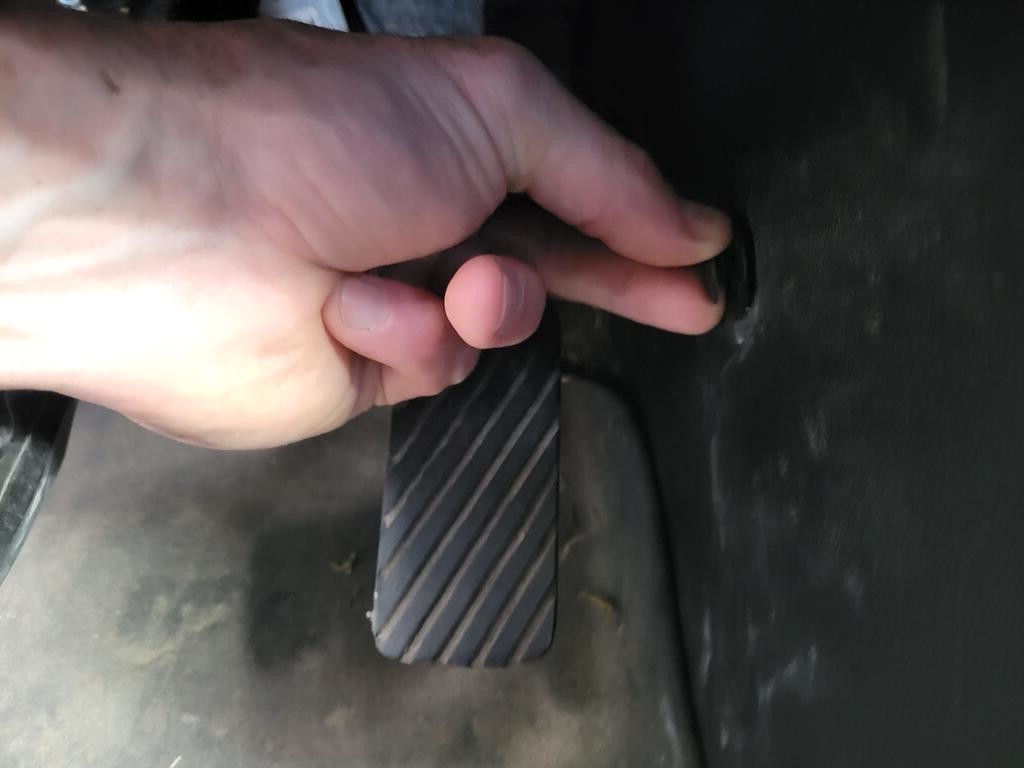
\includegraphics[height=1.5in,angle=0]{photos/usb_trim_clip_left.jpg} } 
  \subfloat[]{\label{subfig:usb_trim:right_clip}
  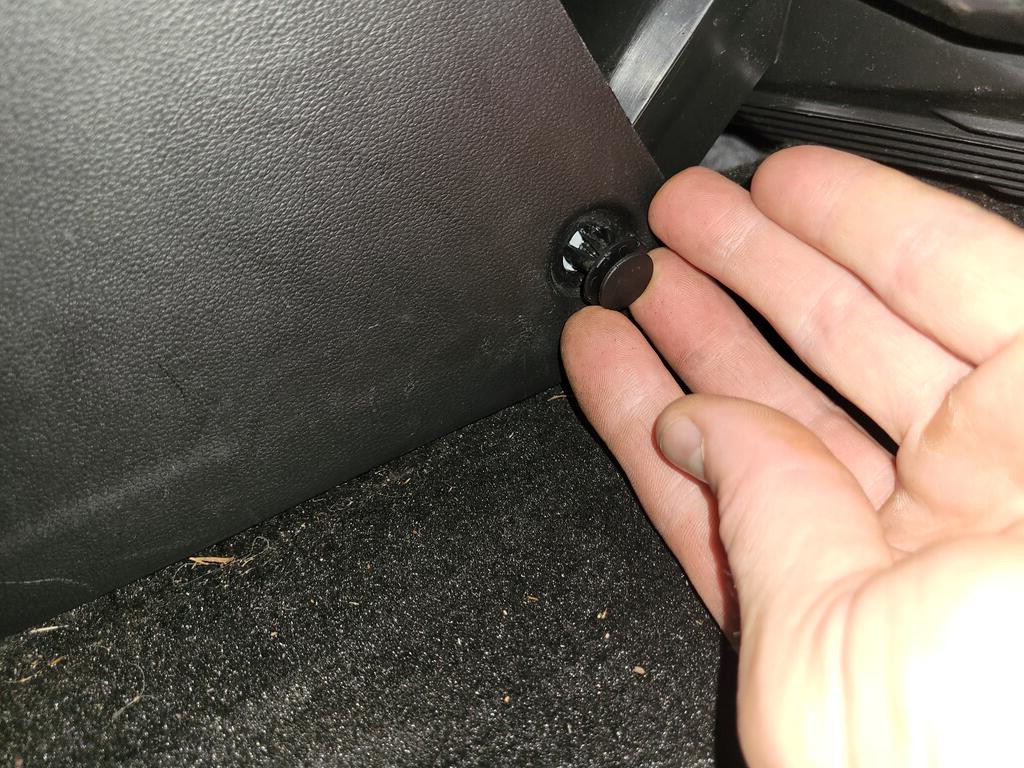
\includegraphics[height=1.5in,angle=0]{photos/usb_trim_clip_right.jpg} } 
  \subfloat[]{\label{subfig:usb_trim:carpet}
  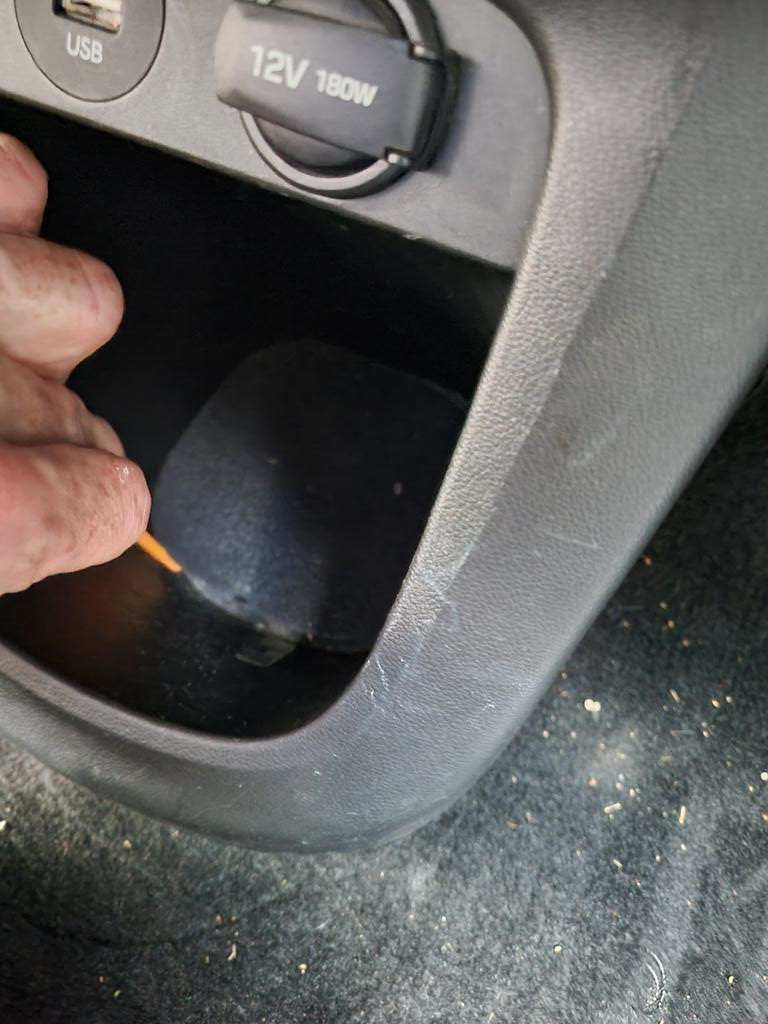
\includegraphics[height=1.5in,angle=0]{photos/removing_usb_trim_carpet.jpg} } \\
  \subfloat[]{\label{subfig:usb_trim:bolt}
  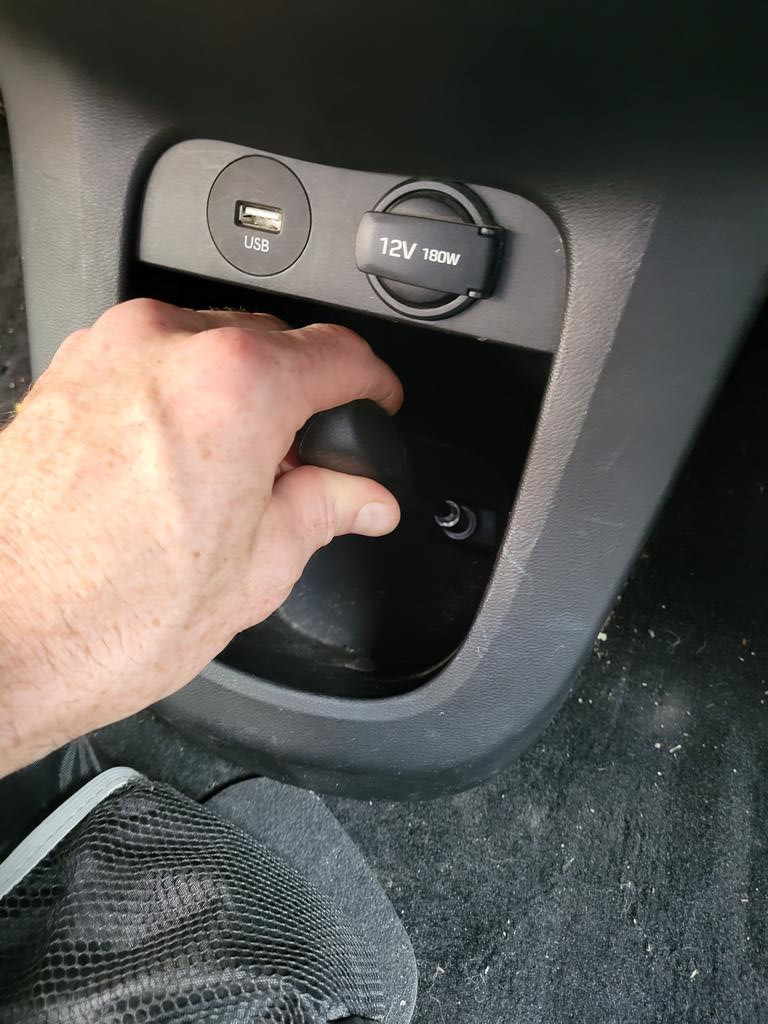
\includegraphics[height=1.5in,angle=0]{photos/removing_usb_trim_bolt.jpg} } 
  \subfloat[]{\label{subfig:usb_trim:trim_off}
  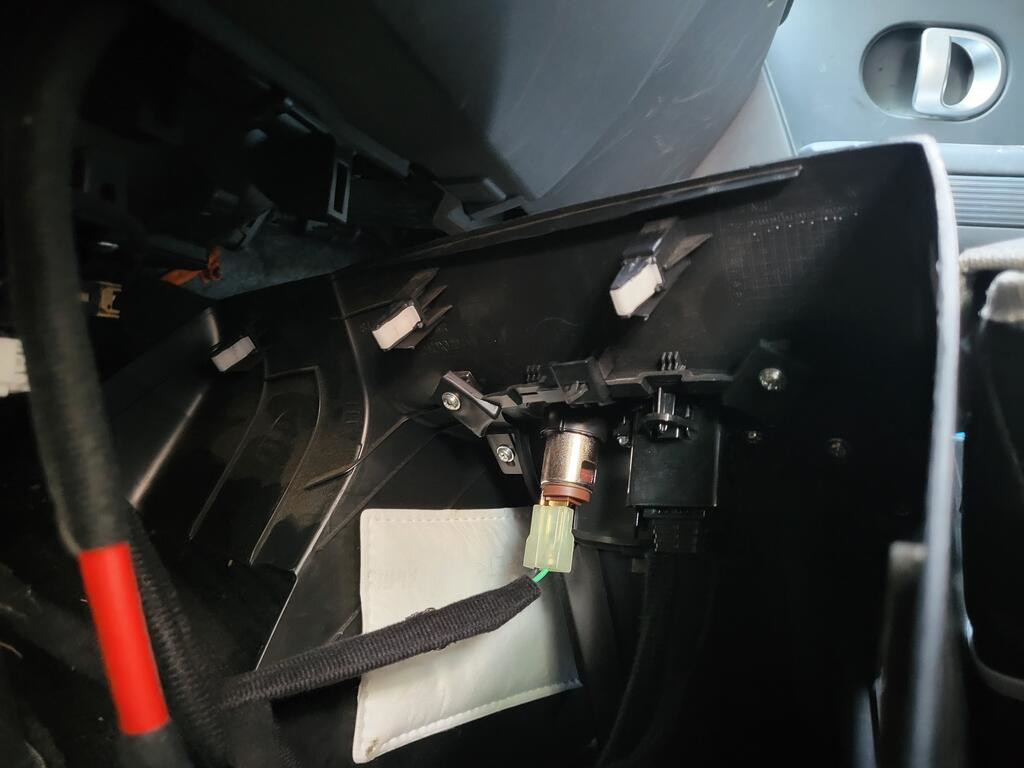
\includegraphics[height=1.5in,angle=0]{photos/usb_trim_off_2.jpg} } 
  \subfloat[]{\label{subfig:usb_trim:trim_to_side}
  \includegraphics[height=1.5in,angle=0]{photos/usb_trim_off.jpg} }  
  \subfloat[]{\label{subfig:usb_trim:HU}
  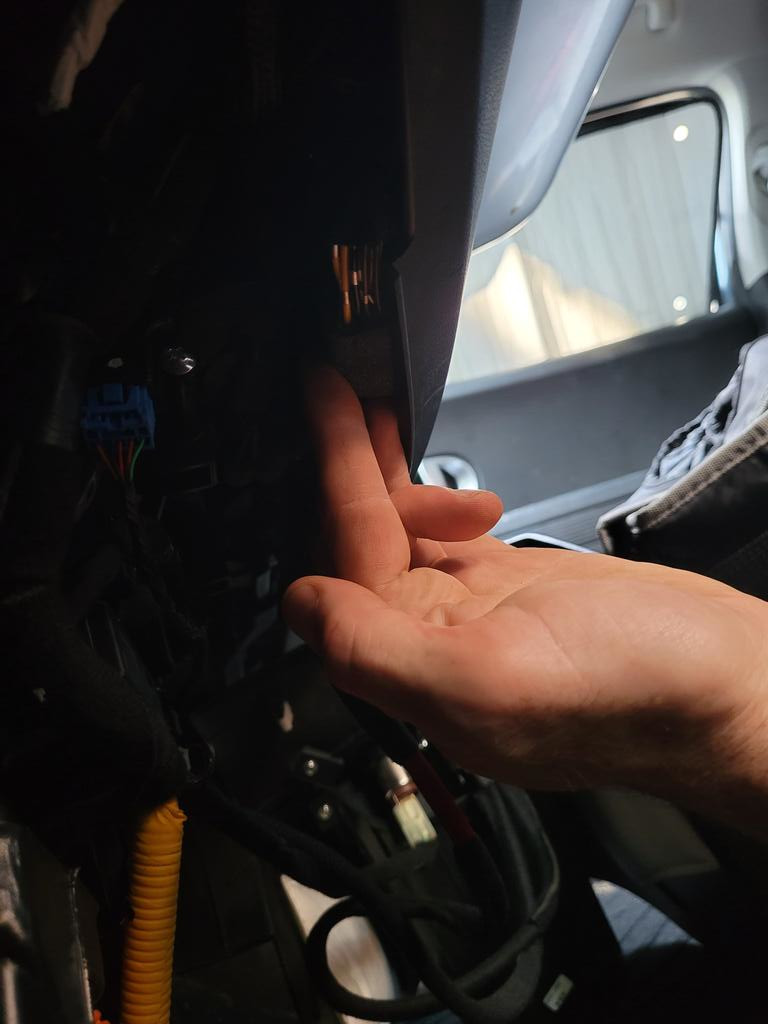
\includegraphics[height=1.5in,angle=0]{photos/usb_trim_off_reaching_for_HU.jpg} } 
   \caption{Ausbau der unteren Ablagefläche in der Mitte: (a) Linke Klammer lösen. (b) Rechte Klammer lösen. (c) Bodenplatte entfernen. (d) Schraube mit 10-mm-Steckschlüssel lösen. (e) Drei Verkleidungsklammern mit dem Verkleidungsdemontagewerkzeug lösen. (f) Verkleidung beiseitelegen. (g) Sie erreichen nun die Unterseite des Autoradios.  \label{fig:usb_trim}}
\end{figure}
\section{Schritt 3: Kabelbaumanschluss} \label{sect:2}
Dieser Schritt umfasst den Einbau des Kabelbaums in das Hauptgerät. 

Schritt-für-Schritt-Anleitung:
\begin{enumerate}
  \item Identifizieren Sie den originalen grauen weiblichen Stecker der Steuereinheit (Abbildung \ref{subfig:harness:headunit})
  \item Entfernen Sie es, indem Sie den Clip zusammendrücken und nach unten ziehen (Abbildung \ref{subfig:harness:M05Bout})
  \item Stecken Sie die weibliche Seite des Kabelbaums in die Kopfeinheit (Abbildung \ref{subfig:harness:female})
  \item Stecken Sie den zuvor entfernten weiblichen Stecker in die männliche Seite des Kabelbaums (Abbildung \ref{subfig:harness:harness_in})
\end{enumerate}

\begin{figure}[h]
  \subfloat[]{\label{subfig:harness:female}
  \includegraphics[height=1.5in,angle=0]{../../../harnesses/head_unit_MITM/photos/labeled_connectors_MITM_harness.jpg} } 
  \subfloat[]{\label{subfig:harness:male}
  \includegraphics[height=1.5in,angle=0]{photos/male_harness_end.jpg} }  \\
  \subfloat[]{\label{subfig:harness:headunit}
  \includegraphics[height=1.5in,angle=0]{photos/head_unit_connectors_in.jpg} } 
  \subfloat[]{\label{subfig:harness:M05Bout}
  \includegraphics[height=1.5in,angle=0]{photos/M05-B_out.jpg} } 
  \subfloat[]{\label{subfig:harness:harness_in}
  \includegraphics[height=1.5in,angle=0]{photos/harness_in.jpg} }  
   \caption{(a) Beschriftetes Foto mit weiblichem Kabelbaumstecker. (b) Männlicher Kabelbaumstecker. (c) Autoradio mit angeschlossenen Steckern. (d) Weiblicher M05-B-Stecker (grau), aus dem Autoradio ausgebaut. (e) Im Autoradio installierter Kabelbaum. \label{fig:harness}}
\end{figure}
\section{Schritt 4: OBD-Halterung} \label{sect:3}
In diesem Schritt montieren wir das OBD-Ende des Kabelbaums sicher und schließen den WiCAN an. 

Schritt-für-Schritt-Anleitung:
\begin{enumerate}
  \item Befestigen Sie den Gurt entlang der Unterkante des unteren Sturzpads
  \item OBD-Buchse in die Halterung einstecken
  \item Befestigen Sie die Halterung mit doppelseitigem Klebeband an der Seite der Fußraumlüftung hinter dem unteren Teil des Sturzpolsters (Abbildung 1). \ref{subfig:obd:wican})
  \item Verwenden Sie Kabelbinder, um den Kabelbaum an anderen Kabeln und Befestigungspunkten zu befestigen (Abbildung \ref{subfig:obd:zip_tie} Und \ref{subfig:obd:zip_tie2})
  \item Halten Sie die Halterung fest und stecken Sie WiCAN ein (Abbildung \ref{subfig:obd:wican})
\end{enumerate}

\begin{figure}[h]
  \subfloat[]{\label{subfig:obd:zip_tie}
  \includegraphics[height=1.5in,angle=0]{photos/zip_tie_1.jpg} } 
  \subfloat[]{\label{subfig:obd:zip_tie2}
  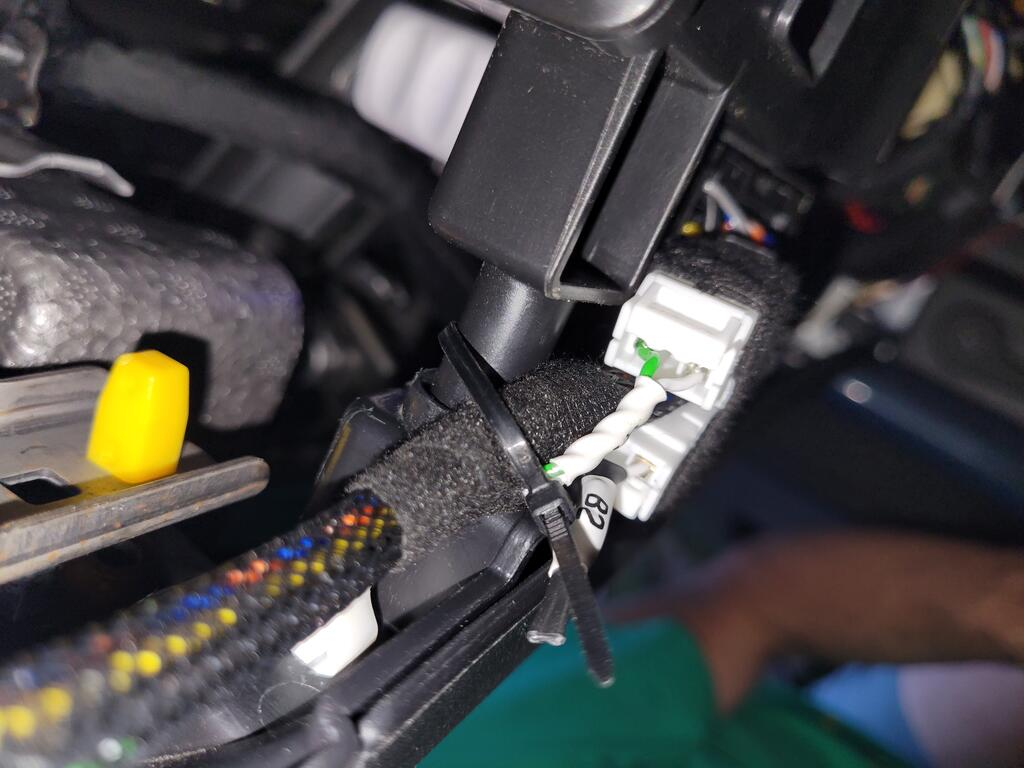
\includegraphics[height=1.5in,angle=0]{photos/harness_mounted_zip_ties_2.jpg} } 
  \subfloat[]{\label{subfig:obd:wican}
  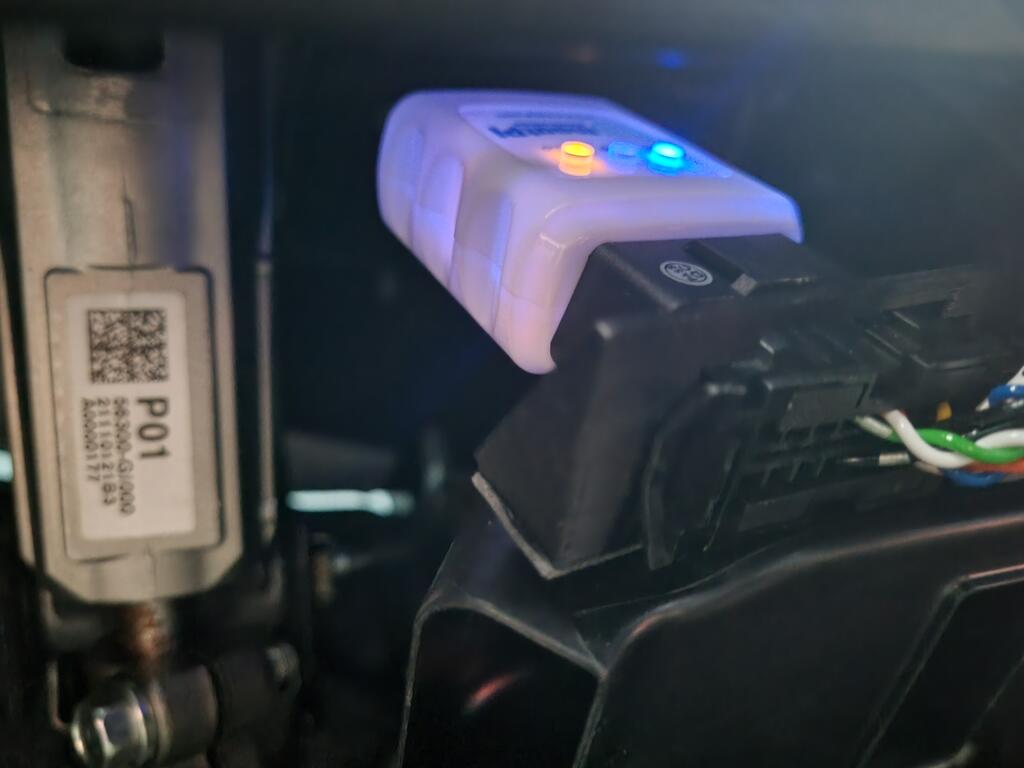
\includegraphics[height=1.5in,angle=0]{photos/WiCAN_installed_on_vent.jpg} } 
   \caption{(a) Kabelbaum mit Kabelbindern an vorhandenem Kabel befestigt. (b) Kabelbaum mit Kabelbindern an der Lüftungshalterung befestigt. (c) WiCAN seitlich an der Lüftungsöffnung montiert. \label{fig:obd}}
\end{figure}

\section{Schritt 5: Aufräumen} \label{sect:4}
Führen Sie die Schritte zum Entfernen der Verkleidung in umgekehrter Reihenfolge aus. Achten Sie darauf, dass die Verkleidungsclips richtig ausgerichtet sind, und drücken Sie die Verkleidungsteile dann fest wieder ein. Schließen Sie den Minuspol der 12-V-Batterie wieder an. Das WiCAN-Gerät sollte sofort blau leuchten. Ändern Sie Ihr WiCAN-Passwort: \href{https://meatpihq.github.io/wican-fw/config/wifi}{https://meatpihq.github.io/wican-fw/config/wifi}Sie können Ihr WiCAN-Gerät direkt verbinden, indem Sie ein WLAN-Netzwerk mit dem Namen „WiCAN“ suchen.\_xxxxxxx' und geht zu \href{http://192.168.80.1/}{http://192.168.80.1/} in Ihrem Browser.
\appendix 
\end{document}
